% questions.tex —— 1987 年·广东卷·文史类 · 题目内容片段（无答案）
% 由 tools/generate_projects.py 依来源总账自 1987/1987_数学真题_广东文_试题.md 生成，勿手改（改源 MD 后重跑）


\gkpart{试题}

\begin{gktip}
\textbf{来源说明}：本题面依据固定源 PDF《附录 I 一九八七年广东省高考数学（文史类）试题与解答》逐题转录。固定源共 16 页，题面为原卷印刷页 265—271，答案与解答为印刷页 272—280；第三大题的解答在固定源中交叉引用印刷页 286，超出本 PDF 范围。

\textbf{图形说明}：第三大题的三棱台图依据固定源图形关系重绘为 TikZ 矢量图。扫描中的断裂线和墨迹粘连不作为额外题设。
\end{gktip}

\begin{question}
\gkti{1}

第一卷共 25 个选择题，每题只有一个结论正确。

（1） $\cos1030^\circ=$

（A）$\cos50^\circ$　　（B）$-\cos50^\circ$　　（C）$\sin50^\circ$　　（D）$-\sin50^\circ$

（2） $2^6$ 与 $0.5^2$ 的等比中项是

（A）$16$　　（B）$\pm4$　　（C）$2$　　（D）$4$

\Needspace{5\baselineskip}
（3） 函数

\nopagebreak[4]
\[
y=\sqrt{2x-x^2}
\]

的定义域是

（A）$(-\infty,0)$　　（B）$(0,2)$　　（C）$[0,2]$　　（D）$[-2,0]$

\Needspace{5\baselineskip}
（4） 指数方程

\nopagebreak[4]
\[
2\cdot4^x-5\cdot2^x+2=0
\]

的解集是

（A）$\{1\}$　　（B）$\{\frac12,1\}$　　（C）$\{-1,\frac12\}$　　（D）$\{-1,1\}$

（5） 下列不等式中，成立的是

（A）$\displaystyle\sin\frac{9\pi}{7}>\sin\frac{8\pi}{7}$

（B）$\displaystyle\cos\frac{9\pi}{7}>\cos\frac{8\pi}{7}$

（C）$\displaystyle\sec\frac{9\pi}{7}>\sec\frac{8\pi}{7}$

（D）$\displaystyle\operatorname{ctg}\frac{9\pi}{7}>\operatorname{ctg}\frac{8\pi}{7}$

（6） 如果圆锥的高和底面直径都等于 $a$，则该圆锥的体积是

（A）$\frac\pi4a^3$　　（B）$\frac\pi6a^3$　　（C）$\frac\pi3a^3$　　（D）$\frac\pi{12}a^3$

\Needspace{5\baselineskip}
（7） 在圆

\nopagebreak[4]
\[
x^2+y^2=4
\]

\Needspace{5\baselineskip}
上，与直线

\nopagebreak[4]
\[
4x+3y-12=0
\]

的距离最小的点的坐标是

（A）$\left(\frac85,\frac65\right)$　　（B）$\left(\frac85,-\frac65\right)$

（C）$\left(-\frac85,\frac65\right)$　　（D）$\left(-\frac85,-\frac65\right)$

（8） 若复数 $z$ 的辐角是 $\frac56\pi$，实部是 $-2\sqrt3$，则 $z=$

（A）$-2\sqrt3-2i$　　（B）$-2\sqrt3+2i$

（C）$-2\sqrt3+2\sqrt3\,i$　　（D）$-2\sqrt3-2\sqrt3\,i$

\Needspace{5\baselineskip}
（9） 已知函数

\nopagebreak[4]
\[
f(x)=x^{\frac13},\qquad g(x)=\left(\frac13\right)^x,
\]

那么，在 $(-\infty,+\infty)$ 上，

（A）$f(x)$ 和 $g(x)$ 都是增函数。

（B）$f(x)$ 和 $g(x)$ 都是减函数。

（C）$f(x)$ 是减函数，而 $g(x)$ 是增函数。

（D）$f(x)$ 是增函数，而 $g(x)$ 是减函数。

\Needspace{5\baselineskip}
（10） 计算下式：

\nopagebreak[4]
\[
\frac{(\sin\alpha+\cos\alpha)^2-(\sin\alpha-\cos\alpha)^2}
{\operatorname{tg}\alpha-\sin\alpha\cos\alpha}
=
\]

（A）$2\operatorname{ctg}^2\alpha$　　（B）$2\operatorname{tg}^2\alpha$

（C）$4\operatorname{ctg}^2\alpha$　　（D）$4\operatorname{tg}^2\alpha$

\Needspace{5\baselineskip}
（11） 函数

\nopagebreak[4]
\[
y=\sin3x+2\cos3x
\]

的最小值是

（A）$-2$　　（B）$-\sqrt5$　　（C）$-3$　　（D）$-5$

\Needspace{5\baselineskip}
（12） 若

\nopagebreak[4]
\[
\operatorname{ctg}\frac\theta2=3,
\]

则 $\cos\theta$ 的值是

（A）$\frac35$　　（B）$-\frac35$　　（C）$-\frac45$　　（D）$\frac45$

\Needspace{5\baselineskip}
（13） 不等式

\nopagebreak[4]
\[
\frac{3x-1}{2-x}\geq1
\]

的解集是

（A）$\left\{x\mid\frac34\leq x\leq2\right\}$

（B）$\left\{x\mid\frac34\leq x<2\right\}$

（C）$\left\{x\mid x>2\ \mathrm{or}\ x\leq\frac34\right\}$

（D）$\{x\mid x<2\}$

\Needspace{5\baselineskip}
（14） 设

\nopagebreak[4]
\[
f(x)=\frac{2x+1}{4x+3}\qquad(x\in R,\ x\ne-\frac34),
\]

\Needspace{5\baselineskip}
则

\nopagebreak[4]
\[
f^{-1}(2)=
\]

（A）$-\frac56$　　（B）$\frac5{11}$　　（C）$\frac25$　　（D）$-\frac25$

（15） 用 $0,1,2,3$ 这四个数字，组成个位数不是 1 的没有重复数字的四位数，共有

（A）16 个　　（B）14 个　　（C）12 个　　（D）10 个

\Needspace{5\baselineskip}
（16） 抛物线

\nopagebreak[4]
\[
y=x^2+3x-2
\]

的对称轴的方程是

（A）$x=\sqrt3$　　（B）$x=-\sqrt3$　　（C）$x=\frac32$　　（D）$x=-\frac32$

\Needspace{5\baselineskip}
（17） 设 $A,B$ 是直线

\nopagebreak[4]
\[
3x+4y+2=0
\]

\Needspace{5\baselineskip}
与圆

\nopagebreak[4]
\[
x^2+y^2+4y=0
\]

的两个交点，则线段 $AB$ 的垂直平分线的方程是

（A）$3y-4x+2=0$　　（B）$3y-4x+6=0$

（C）$3y+4x+6=0$　　（D）$4y+3x+8=0$

\Needspace{5\baselineskip}
（18） 椭圆

\nopagebreak[4]
\[
x^2+4y^2+4x=0
\]

的右焦点的坐标是

（A）$(\sqrt3-2,0)$　　（B）$(\sqrt3+2,0)$

（C）$(\sqrt3,0)$　　（D）$(-\sqrt3,0)$

（19） 设双曲线的半焦距为 $c$，两条准线的距离为 $d$，且 $c=d$，则这双曲线的离心率 $e=$

（A）$\sqrt3$　　（B）$\sqrt2$　　（C）$2$　　（D）$3$

\Needspace{5\baselineskip}
（20） 若

\nopagebreak[4]
\[
\theta\in\left(\frac\pi2,\frac34\pi\right),
\]

\Needspace{5\baselineskip}
则

\nopagebreak[4]
\[
\frac{x^2}{\csc\theta-2}+\frac{y^2}{2-\sec\theta}=1
\]

所表示的曲线是

（A）焦点在 $x$ 轴上的椭圆。

（B）焦点在 $y$ 轴上的椭圆。

（C）焦点在 $x$ 轴上的双曲线。

（D）焦点在 $y$ 轴上的双曲线。

（21） 若正三棱锥的一个侧面的面积与底面的面积的比等于 $\frac23$，则这个三棱锥的侧面和底面所成的二面角是

（A）$15^\circ$　　（B）$30^\circ$　　（C）$45^\circ$　　（D）$60^\circ$

（22） 设 $\alpha$ 和 $\beta$ 是两个不重合的平面，$l$ 和 $m$ 是两条不重合的直线，则 $\alpha\parallel\beta$ 的一个充分条件是

（A）$l\subset\alpha,\ m\subset\alpha$，且 $l\parallel\beta,\ m\parallel\beta$。

（B）$l\subset\alpha,\ m\subset\beta$，且 $l\parallel m$。

（C）$l\perp\alpha,\ m\perp\beta$，且 $l\parallel m$。

（D）$l\parallel\alpha,\ m\parallel\beta$，且 $l\parallel m$。

（23） 如果实数 $a,b,c$ 不全为零，那么

（A）实数 $a,b,c$ 中，至少有一个正数。

（B）实数 $a,b,c$ 中，既有正数又有负数。

（C）实数 $a,b,c$ 的乘积不是零。

（D）实数 $a,b,c$ 中，至多有两个零。

\Needspace{5\baselineskip}
（24） 已知函数

\nopagebreak[4]
\[
f(x)=\sin\left(\frac34x+\frac52\pi\right),
\qquad
g(x)=\lg\left(\sqrt{x^2+1}-x\right),
\]

则

（A）$f(x)$ 是奇函数，而 $g(x)$ 既不是奇函数，又不是偶函数。

（B）$f(x)$ 是偶函数，而 $g(x)$ 是奇函数。

（C）$f(x)$ 和 $g(x)$ 都是奇函数。

（D）$f(x)$ 是偶函数，而 $g(x)$ 既不是奇函数，又不是偶函数。

\Needspace{5\baselineskip}
（25） 若等差数列的第一、二、三项依次是

\nopagebreak[4]
\[
\frac1{x+1},\qquad \frac5{6x},\qquad \frac1x,
\]

那么，这个等差数列的第 101 项的值是

（A）$50\frac13$　　（B）$13\frac23$　　（C）$24$　　（D）$8\frac23$

\end{question}
\begin{question}
\gkti{2}

第二卷第一题（本题满分 15 分）共有五个填空小题，每小题 3 分。

\Needspace{5\baselineskip}
（1） 若

\nopagebreak[4]
\[
z=\sqrt2+i,
\]

则 $z^2$ 的共轭复数的代数形式是 $\underline{\hspace{3em}}$。

（2） 已知椭圆的两个焦点是 $F_1(-2,0),F_2(2,0)$，并且点 $A(0,2)$ 在该椭圆上，那么，这个椭圆的标准方程是 $\underline{\hspace{5em}}$。

\Needspace{5\baselineskip}
（3） 计算极限：

\nopagebreak[4]
\[
\lim_{n\to\infty}\frac{4n^3-1}{n(2n^2+1)}
\]

的值是 $\underline{\hspace{3em}}$。

\Needspace{5\baselineskip}
（4） 设

\nopagebreak[4]
\[
(1-x)^7=a_0+a_1x+a_2x^2+a_3x^3+a_4x^4+a_5x^5+a_6x^6+a_7x^7,
\]

\Needspace{5\baselineskip}
则

\nopagebreak[4]
\[
a_0+a_2+a_4+a_6
\]

的值是 $\underline{\hspace{3em}}$。

\Needspace{5\baselineskip}
（5） 函数

\nopagebreak[4]
\[
y=\frac{2x}{1+x^2}\qquad(x\in R)
\]

的值域是 $\underline{\hspace{3em}}$。

\end{question}
\begin{question}
\gkti{3}

\Needspace{5\baselineskip}
第二卷第二题（本题满分 12 分）。设正数 $a,b,c$ 满足

\nopagebreak[4]
\[
a^2+b^2=c^2.
\]

\Needspace{5\baselineskip}
（1） 求证：

\nopagebreak[4]
\[
\log_2\left(1+\frac{b+c}{a}\right)
+\log_2\left(1+\frac{a-c}{b}\right)=1.
\]

\Needspace{5\baselineskip}
（2） 又设

\nopagebreak[4]
\[
\log_4\left(1+\frac{b+c}{a}\right)=1,\qquad
\log_8(a+b-c)=\frac23,
\]

求 $a,b,c$ 的值。

\Needspace{0.4\textheight}
\end{question}
\begin{question}
\gkti{4}

\Needspace{5\baselineskip}
第二卷第三题（本题满分 14 分）。在三棱台

\nopagebreak[4]
\[
A_1B_1C_1-ABC
\]

\Needspace{5\baselineskip}
中，侧棱 $B_1B\perp$ 底面 $ABC$，且

\nopagebreak[4]
\[
\angle ABC=\angle AA_1C=\frac\pi2,\qquad
AB=2A_1B_1=2\text{ cm}.
\]
\nopagebreak[4]
\begin{center}% 1987 年广东卷文史类第三大题：三棱台
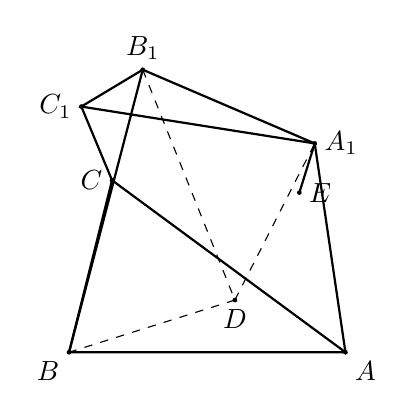
\begin{tikzpicture}[scale=0.78,>=stealth]
  \coordinate (A) at (4.5,0);
  \coordinate (B) at (0,0);
  \coordinate (C) at (0.7,2.8);
  \coordinate (A1) at (4.0,3.4);
  \coordinate (B1) at (1.2,4.6);
  \coordinate (C1) at (0.2,4.0);
  \coordinate (D) at (2.7,0.85);
  \coordinate (E) at (3.75,2.6);
  \draw[thick] (A)--(B)--(C)--(A);
  \draw[thick] (A1)--(B1)--(C1)--(A1);
  \draw[thick] (A)--(A1) (B)--(B1) (C)--(C1);
  \draw[dashed] (B1)--(D) (D)--(A1) (D)--(B);
  \draw[thick] (E)--(A1);
  \fill (A) circle (1.1pt) node[below right] {$A$};
  \fill (B) circle (1.1pt) node[below left] {$B$};
  \fill (C) circle (1.1pt) node[left] {$C$};
  \fill (A1) circle (1.1pt) node[right] {$A_1$};
  \fill (B1) circle (1.1pt) node[above] {$B_1$};
  \fill (C1) circle (1.1pt) node[left] {$C_1$};
  \fill (D) circle (1.1pt) node[below] {$D$};
  \fill (E) circle (1.1pt) node[right] {$E$};
\end{tikzpicture}
\end{center}
\nopagebreak[4]
（1） 求证：$BC\perp A_1B,\ BC\perp A_1A,\ A_1A\perp A_1B$。

（2） 求异面直线 $A_1A$ 和 $BC$ 的距离。

\end{question}
\begin{question}
\gkti{5}

\Needspace{5\baselineskip}
第二卷第四题（本题满分 15 分）。直线 $l$ 通过抛物线

\nopagebreak[4]
\[
y^2=2px\qquad(p\ne0)
\]

的焦点，并且与这抛物线相交于 $A(x_1,y_1)$ 和 $B(x_2,y_2)$ 两点。

\Needspace{5\baselineskip}
（1） 求证：

\nopagebreak[4]
\[
y_1y_2=-p^2.
\]

（2） 点 $C$ 在这条抛物线的准线上，且 $AC$ 平行于 $x$ 轴，求证：$B,C$ 和这条抛物线的顶点三点共线。

\end{question}
\begin{question}
\gkti{6}

\Needspace{5\baselineskip}
第二卷第五题（本题满分 14 分）。设 $|\theta|<\frac\pi2$，数列 $\{a_n\}$ 的通项是

\nopagebreak[4]
\[
a_n=\sin\frac{n\pi}{2}\cdot\operatorname{tg}^n\theta,
\]

\Needspace{5\baselineskip}
记

\nopagebreak[4]
\[
S_{2n}=a_1+a_2+\cdots+a_{2n-1}+a_{2n}.
\]

\Needspace{5\baselineskip}
（1） 求证：对任何自然数 $n$，

\nopagebreak[4]
\[
S_{2n}=\frac12(\sin2\theta)
\left[1+(-1)^{n+1}\operatorname{tg}^{2n}\theta\right].
\]

\Needspace{5\baselineskip}
（2） 求证：当 $n\ge2$ 时，

\nopagebreak[4]
\[
a_n^2+a_{n-1}\cdot a_{n+1}+(-1)^n(a_1)^{2n}=0.
\]

\end{question}